\section{Método de Runge-Kutta de Grado 4}

El método más utilizado de los Runge-Kutta es el de grado 4, frecuentemente conocido como «RK4»; incluso algunas veces es simplemente llamado \textit{el} método de Runge-Kutta.

\subsection{Funcionamiento de RK4}\label{sect:def-rk4}

Sea la siguiente ecuación diferencial:
\begin{equation} \label{eq:main-diff-eq}
	\frac{dy}{dt} = f(t,y)
\end{equation}
…con la condición de valor inicial:
\begin{equation*}
	y(t_0) = y_0
\end{equation*}
Aquí conocemos \(f\) y las condiciones inicales \(t_0, y_0\), deseando aproximar a \(y\), una función desconocida sobre \(t\). Utilizaremos el método RK4 para obtener esta aproximación.

Antes que nada, debemos:
\begin{itemize}
	\item Definir el intervalo para \(t\) sobre el cual estaremos aproximando la solución.
	\item Definir el tamaño \(h\) de los pasos por iteración que estaremos tomando sobre ese intervalo.
\end{itemize}
El número de iteraciones que realizaremos dependerá de la razón entre el intervalo para \(t\) y el tamaño \(h\) que elijamos. Aquí, estamos básicamente convirtiendo el intervalo continuo de \(t\) en uno discreto a través de \(h\), sobre el cual estaremos iterando en el método.

Comenzamos definiendo los dos valores más importantes que se estarán determinando durante cada iteración \(n \in [0, 1, 2, \dots]\):
\begin{align}
	y_{n+1} &= y_{n} + \frac{h}{6} \left( k_{1} + 2k_{2} + 2k_{3} + k_{4} \right) \label{eq:weighted-avg} \\[0.5em]
	t_{n+1} &= t_{n} + h \nonumber
\end{align}
Es en la definición de \(y_{n+1}\) que se nos presentan los valores \(k_{1}, k_{2}, k_{3}, k_{4}\), que son los que caracterizan al método RK4 y donde realizaremos la mayor cantidad de cálculos involucrados. Estos cuatro valores se definen para cada iteración \(n\) como:
\begin{align}
	k_{1} &= f(t_{n}, y_{n}) \label{eq:k1} \\
	k_{2} &= f \left( t_{n} + \frac{h}{2}, y_{n} + h \frac{k_{1}}{2} \right) \label{eq:k2} \\
	k_{3} &= f \left( t_{n} + \frac{h}{2}, y_{n} + h \frac{k_{2}}{2} \right) \label{eq:k3} \\
	k_{4} &= f(t_{n} + h, y_{n} + hk_{3}) \label{eq:k4}
\end{align}

\subsection{Visualización de K4}

Puede que hasta el momento la descripción anterior del método de Runge-Kutta de grado 4 (RK4) haya parecido bastante abstracta, pero describámosla y visualicémosla para que su funcionamiento quede más claro.

\begin{figure}[H]\label{fig:slopes}
	\centering
	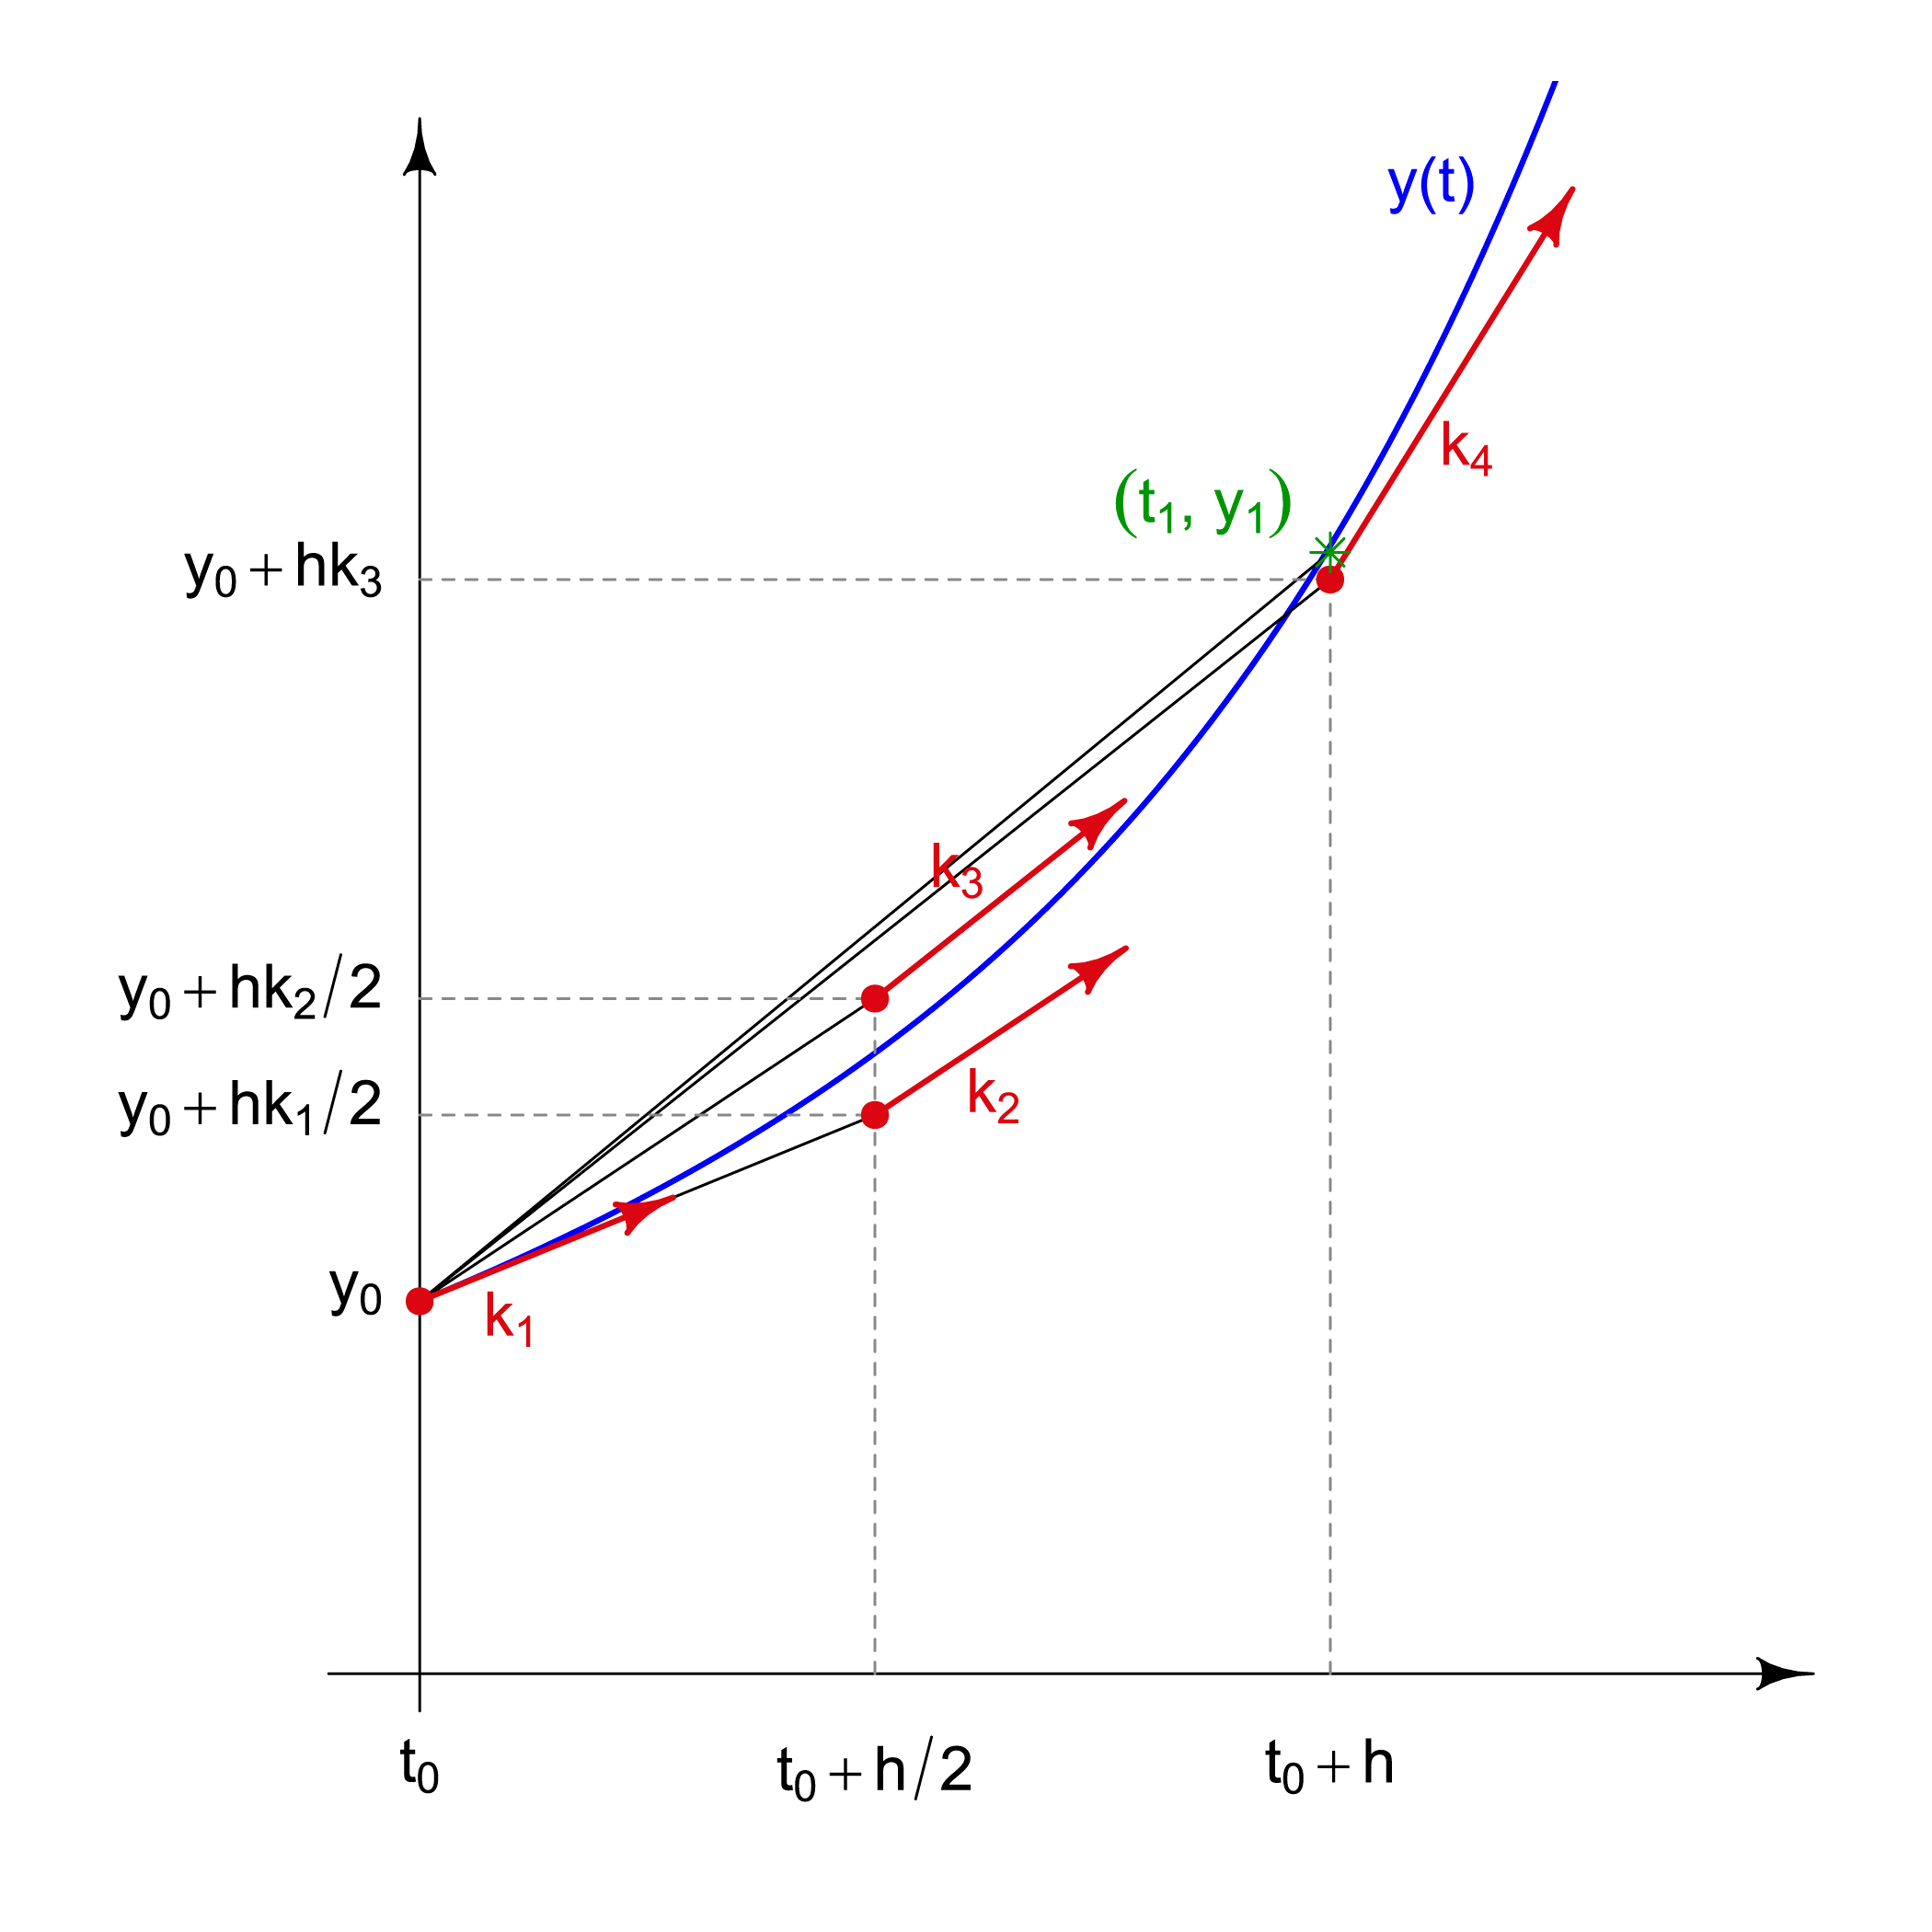
\includegraphics[scale=0.6]{../auxiliary/assets/Runge-Kutta_slopes.png}
	\caption{Aproximación de la solución a \(\frac{dy}{dt} = y + t^{3}\) con \(y_{0}\) y un intervalo para \(t\) arbitrarios. En azul, la solución exacta; en rojo, las pendientes correspondientes a los valores \(k_{i}\); en verde, uno de los puntos de la solución, que corresponde a la aproximación obtenida durante la primera iteración con paso \(h\). Gráfico obtenido de \url{https://en.wikipedia.org/wiki/File:Runge-Kutta_slopes.svg}.}
\end{figure}
La figura~\ref{fig:slopes} representa el funcionamiento de RK4 para la obtención de la solución a la ecuación diferencial \(\frac{dy}{dt} = y + t^{3}\) bajo la condición \(y(t_{0}) = y_{0}\), con \(y_{0}\) y el intervalo para \(t\) arbitrarios.

La obtención analítica de la solución exacta para esta ecuación diferencial es, de hecho, posible y es por ello por lo que pudo ser trazada como la línea azul, por lo que estrictamente hablando no es necesaria la implementación de un método numérico para obtenerla. Sin embargo, se ha utilizado simplemente para ejemplificar y visualizar el funcionamiento del método RK4.

\subsubsection{Pendientes a lo Largo del Intervalo}

Lo primero que notamos es que los valores \(k_{i}\) representan pendientes. Si regresamos a su definición en la sección anterior ((\ref{eq:k1}), (\ref{eq:k2}), (\ref{eq:k3}) y (\ref{eq:k4})), notamos que son simplemente evaluaciones de \(f(t,y)\) en valores concretos para \(t\) y \(y\), y que la ecuación diferencial de la que partimos establece que esa función describe la derivada (véase (\ref{eq:main-diff-eq})), por lo que la razón de ser de este resultado se vuelve evidente.

Analizando un poco más las definiciones de estas \(k_{i}\), y con ayuda de la figura~\ref{fig:slopes}, notaremos también que estas pendientes no son del todo arbitrarias:
\begin{itemize}
	\item \(k_{1}\) es la pendiente al inicio del intervalo.
	\item \(k_{2}\) es la pendiente en el punto medio del intervalo (de ahí que involucre \(\frac{h}{2}\)), apoyándose de \(k_{1}\).
	\item \(k_{3}\), similar a \(k_{2}\), es la pendiente en el punto medio del intervalo, pero esta vez apoyándose de \(k_{2}\).
	\item \(k_{4}\) es la pendiente al final del intervalo
\end{itemize}

\subsubsection{Aproximación Obtenida}

Al final de cada iteración \(n\) obtenemos \(y_{n+1}\), que no es más que la aproximación de \(y(t_{n+1})\) según el método.

Notemos que este valor es determinado por la \(y_{n}\) actual correspondiente a la iteración, sumada con una media ponderada de cuatro incrementos, cada uno correspondiendo al producto de las cuatro pendientes anteriormente descritas por la longitud del paso \(h\). Esta media ponderada favorece sobre todo a las pendientes \(k_{2}\) y \(k_{3}\), las del medio del intervalo.

Visto de otra forma, las pendientes \(k_{i}\) descritas anteriormente van guiando al método a lo largo del intervalo, lo que le permite obtener una aproximación relativamente precisa de un punto de la solución al final de él.
